% Provenance (never printed): old terminale S material on magmatism in
% subduction zones (volcanic arcs above the slab, water released by the slab
% and hydrous melting of the mantle wedge, andesitic volcanism and granitoid
% plutons, growth of the continental crust). Owner (Sync 0): volcanic arc,
% hydrous melting, granodiorite, batholith, continental growth. Subduction,
% slab, Wadati-Benioff zone, blueschist and eclogite are g11.06's; partial and
% decompression melting and peridotite g11.05's; andesite, diorite, rhyolite,
% pluton g11.08's; continental crust g12.01's; magma, explosive eruption Book 1's
% (g7): recalled, never redefined. Figures: figdata/grade-12/arc_magmatism.py
% (GVP volcanoes, ComCat NE Japan band, dry solidus via grade-11
% geotherm_solidus.py, wet solidus brackets of Wang 2020 and Kawamoto-Holloway 1997).
\chapter{Magmatism at Subduction Zones}\label{ch:g12:subduction-magmatism}

On 18 May 1980, at 8:32 in the morning, a magnitude 5.1 earthquake shook
Mount St.~Helens. At once the north flank of the volcano, which had been
bulging outwards by about two metres a day, slid away: the largest debris
avalanche in recorded history, about \qty{2.5}{km^3} of rock. Freed of its
load, the gas-rich magma inside blew out sideways through the scar, at no
less than \qty{480}{km/h}, flattening forests over \qty{600}{km^2}. Within
fifteen minutes a column of ash stood more than \qty{24}{km} high, and the
eruption went on for nine hours. Sixty-one people were killed or never found.
% ledger: usgs:b2-msh-1980, usgs:msh-deaths

\begin{omfigure}
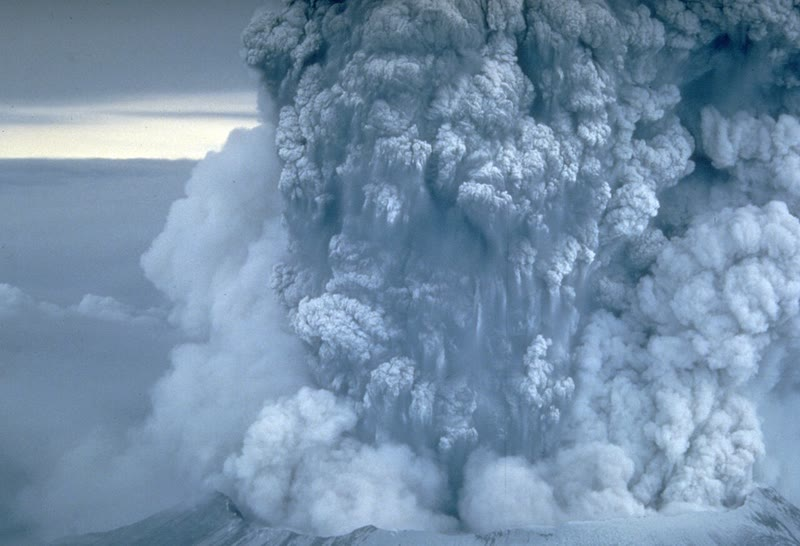
\includegraphics[width=0.55\linewidth]{images/book2/g12-swanson-st-helens-plume.jpg}

{\small The ash column of Mount St.~Helens on 18 May 1980, which rose more
than \qty{24}{km} in less than fifteen minutes. Photograph Donald
A.~Swanson, USGS (public domain).}
\end{omfigure}
% ledger: photo:g12-st-helens, usgs:b2-msh-1980

Mount St.~Helens is one of a line of volcanoes --- Baker, Rainier, Hood,
Shasta and others --- that stands above the place where a small oceanic
plate, the Juan de Fuca Plate, sinks beneath North America. This chapter
asks why volcanoes are found there, why their eruptions are so often violent,
and what becomes of the magma that never reaches the surface.
% ledger: earle:cascades

\begin{recall}
At a \omterm{def:g11:subduction-zones:subduction}{subduction zone}, a plate of \omterm{def:g11:ocean-ridges:oceanic-lithosphere}{oceanic lithosphere} sinks back into the
mantle beneath another plate; its earthquakes, the \omterm{def:g11:subduction-zones:benioff}{Wadati--Benioff zone},
trace the \omterm{def:g11:subduction-zones:slab}{slab} down to as deep as \qty{670}{km}
(\cref{ch:g11:subduction-zones}). The mantle is made of \omterm{def:g11:ocean-ridges:peridotite}{peridotite}; it is
solid, but a rock that rises and is less squeezed may melt in part, by
\omterm{def:g11:ocean-ridges:partial-melting}{decompression melting}, as beneath a ridge (\cref{ch:g11:ocean-ridges}).
\omterm{def:g11:igneous-rocks:rock-names}{Andesite} is a \omterm{def:g11:igneous-rocks:volcanic-plutonic}{volcanic rock} between basalt and \omterm{def:g11:igneous-rocks:rock-names}{rhyolite}, \omterm{def:g11:igneous-rocks:rock-names}{diorite} its \omterm{def:g11:igneous-rocks:volcanic-plutonic}{plutonic}
equivalent, and a \omterm{def:g11:igneous-rocks:intrusion}{pluton} a large body of magma that cooled underground
(\cref{ch:g11:igneous-rocks}). The \omterm{def:g12:continental-crust:continental-crust}{continental crust} is thick and light,
mostly granitic rock on top (\cref{ch:g12:continental-crust}). An explosive
eruption blows the magma to pieces with its own gas (Book 1, grade 7).
\end{recall}
% ledger: tulane:magma-types, tulane:intrusions, rg14:crust

\section{Volcanic arcs}

Most of the active volcanoes on land do not stand at random. Of the 1214
volcanoes that have erupted since the end of the last ice age and are listed
in the catalogue of the Global Volcanism Program, 838 --- more than two out
of three --- stand above a \omterm{def:g11:subduction-zones:subduction}{subduction zone}. Around the Pacific they make an
almost unbroken ring, often called the Ring of Fire, and every line of them
runs parallel to a trench, on the side of the plate that does not sink.
% values: n_volcanoes 1214, n_subduction 838, frac_subduction 0.690 (arc_magmatism.py)
% ledger: data:gvp, tulane:arc

\begin{omfigure}
\begin{tikzpicture}
\begin{axis}[ommap, width=\linewidth, xtick={-180,-90,...,180}, ytick={-60,0,60},
  legend style={font=\scriptsize, at={(0.5,-0.13)}, anchor=north, legend columns=3,
    /tikz/every even column/.append style={column sep=6pt}}]
\addplot[fill=omLithAlluv, draw=black!45, line width=0.2pt, forget plot] table {figdata/out/shared-geo-land.dat};
\addplot[black!70, line width=0.5pt, forget plot] table {figdata/out/shared-geo-school-subduction.dat};
\addplot[fill=black!70, draw=none, forget plot] table {figdata/out/shared-geo-school-teeth.dat};
% computed in figdata/grade-12/arc_magmatism.py; ledger: data:gvp, data:pb2002, data:ne-land
\addplot[only marks, mark=triangle*, mark size=1.1pt, black!40] table[x=lon, y=lat] {figdata/out/grade-12-arc_magmatism-world-other.dat};
\addplot[only marks, mark=triangle*, mark size=1.3pt, omThm] table[x=lon, y=lat] {figdata/out/grade-12-arc_magmatism-world-sub.dat};
\addlegendimage{black!70, line width=0.5pt}
\legend{{other volcanoes}, {volcanoes above a subduction zone}, {trench}}
\end{axis}
\end{tikzpicture}

{\small The volcanoes active since the end of the last ice age, red where
they stand above a \omterm{def:g11:subduction-zones:subduction}{subduction zone}, with the trenches (black line, triangles
on the plate that overrides). Data: Smithsonian Global Volcanism Program;
plate boundaries of Bird (2003); land from Natural Earth.}
\end{omfigure}
% values: n_subduction 838 of 1214 (arc_magmatism.py)

\begin{definition}[Volcanic arc]\label{def:g12:subduction-magmatism:arc}
A \emph{volcanic arc}\index{volcanic arc} is a line of volcanoes on the
overriding plate of a \omterm{def:g11:subduction-zones:subduction}{subduction zone}, parallel to the trench, standing
above the place where the \omterm{def:g11:subduction-zones:slab}{slab} has reached a depth of about a hundred
kilometres. It is an \emph{island arc} when it rises from the sea floor, as
in Japan or Indonesia, and a continental arc when it stands on a continent,
as in the Andes or the Cascades.
\end{definition}
% ledger: tulane:arc, earle:arc-water, earle:cascades, sa06:slab-depth

The edge of the arc nearest the trench is called the \textbf{volcanic
front}: on the trench side of it, there are no volcanoes at all. How deep is
the \omterm{def:g11:subduction-zones:slab}{slab} beneath it?

\begin{proposition}[The slab beneath the volcanic front]\label{prop:g12:subduction-magmatism:depth}
If the \omterm{def:g11:subduction-zones:slab}{slab} is a plane that dips at an angle $\theta$ from the trench, and
the volcanic front lies at a horizontal distance $d$ from the trench, then
the top of the \omterm{def:g11:subduction-zones:slab}{slab} lies beneath the front at a depth
\[
  H = d \tan\theta .
\]
\end{proposition}

\begin{proof}
Take a vertical section across the trench. The \omterm{def:g11:subduction-zones:slab}{slab}, the surface and the
vertical line beneath the front make a right triangle, with the right angle
beneath the front: the side along the surface is $d$, the vertical side is
$H$, and the angle at the trench is $\theta$. So $\tan\theta = H/d$.
\end{proof}

A compilation of 839 volcanic centres along \qty{33000}{km} of arcs measured
$H$ beneath each of them: averaged over stretches of arc \qty{500}{km} long,
it ranges from 72 to \qty{173}{km}, with a mean of \qty{105}{km}. Arcs above
steep \omterm{def:g11:subduction-zones:slab}{slabs} lie close to their trench, arcs above gently dipping \omterm{def:g11:subduction-zones:slab}{slabs} far
from it, but the \omterm{def:g11:subduction-zones:slab}{slab} beneath them is always about a hundred kilometres
down.
% ledger: sa06:slab-depth

\begin{method}[Finding the slab under a volcano]\label{met:g12:subduction-magmatism:slab}
\begin{enumerate}
  \item Take the earthquakes of a narrow band across the arc, and plot their
        depth against their distance across it, at true scale.
  \item Keep the earthquakes deeper than about \qty{70}{km}: shallower ones
        also occur in the overriding plate and on the fault between the two
        plates.
  \item Draw the line, or read the depth, of the deep earthquakes beneath
        the volcanic front: that is the depth of the \omterm{def:g11:subduction-zones:slab}{slab} there.
  \item Check it with $H = d\tan\theta$, measuring $d$ from the trench and
        the dip $\theta$ on the section.
\end{enumerate}
\end{method}

\begin{omfigure}
\begin{tikzpicture}
\begin{axis}[omsection, name=jp, scale only axis, width=0.8\linewidth, height=0.2857\linewidth,
  xmin=0, xmax=700, ymin=0, ymax=250, y dir=reverse,
  xlabel={distance east of \ang{138}~E (\unit{km})}, ylabel={depth (\unit{km})},
  xtick={0,100,...,700}, ytick={0,50,...,250}, tick label style={font=\small},
  every axis label/.append style={font=\small}]
% computed in figdata/grade-12/arc_magmatism.py; ledger: data:b2-usgs-ne-japan, data:gvp, data:pb2002
\addplot[only marks, mark=*, mark size=0.55pt, black!35] table[x=x_km, y=depth] {figdata/out/grade-12-arc_magmatism-jp-quakes.dat};
\addplot[omDef, line width=0.9pt, dashed] table[x=x_km, y=depth] {figdata/out/grade-12-arc_magmatism-jp-slab.dat};
\addplot[only marks, mark=triangle*, mark size=2.6pt, omThm] table[x=x_km, y expr=-7] {figdata/out/grade-12-arc_magmatism-jp-volc.dat};
\draw[omThm, densely dotted, line width=0.8pt] (axis cs:259.2,0) -- (axis cs:259.2,98.2);
\fill[omThm] (axis cs:259.2,98.2) circle (1.6pt);
\coordinate (front) at (axis cs:259.2,-14);
\coordinate (trench) at (axis cs:528.9,-14);
\coordinate (H) at (axis cs:262,60);
\coordinate (slab) at (axis cs:95,228);
\draw[black, line width=0.9pt] (axis cs:528.9,-12) -- (axis cs:528.9,0);
\end{axis}
\node[font=\scriptsize, anchor=south, text=omThm] at (front) {volcanic front (Iwate)};
\node[font=\scriptsize, anchor=south] at (trench) {Japan Trench};
\node[font=\scriptsize, anchor=west, text=omThm, fill=white, inner sep=1pt] at (H) {\qty{98}{km}};
\node[font=\scriptsize, anchor=west, text=omDef, fill=white, inner sep=1pt] at (slab) {slab, dipping about \ang{20}};
\end{tikzpicture}

{\small A section across north-east Japan at true scale: the earthquakes of
magnitude 4.5 or more between \ang{37.5} and \ang{40.5}~N, 1976--2025 (grey),
the volcanoes of the same band (red triangles) and the line fitted to the
earthquakes deeper than \qty{70}{km} (blue, dashed). Two out of five of the
shallow events east of \ang{141.5}~E date from 2011, the year of the great
earthquake of March. Data: USGS
earthquake catalogue; Smithsonian Global Volcanism Program; plate boundaries
of Bird (2003).}
\end{omfigure}
% values: shallow (<70 km) events east of 141.5 E: 3622, of which 1451 in 2011 (0.40); ledger usgs:tohoku
% values: jp_front_lon 141.0 (x 259.2 km), jp_trench_lon 144.12 (x 528.9), jp_front_trench_km 269.4, jp_dip_deg 19.98, jp_H_geom 98.0, bin_141_median 98.15, jp_slab_depth_front 105.6 (arc_magmatism.py)

\begin{example}[North-east Japan]\label{ex:g12:subduction-magmatism:japan}
In the band of the figure, the easternmost volcano is Iwate, at \ang{141.0}~E,
and the Japan Trench lies at \ang{144.1}~E. One degree of longitude there is
$111.2\cos\ang{39} \approx \qty{86.4}{km}$, so $d \approx 3.12 \times 86.4
\approx \qty{270}{km}$. The deep earthquakes dip at about \ang{20}, and
\[
  H = 270 \times \tan\ang{20} \approx \qty{98}{km}.
\]
The earthquakes deeper than \qty{70}{km} that lie beneath the front itself
have a median depth of \qty{98}{km}: the two agree, close to the world
average.
\end{example}
% values: km_per_deg_lon 86.415, jp_front_trench_km 269.4, jp_dip_deg 19.98, jp_H_geom 97.98, bin_141_median 98.15 (arc_magmatism.py)

\section{Water melts the mantle}

Beneath an arc, the \omterm{def:g11:subduction-zones:slab}{slab} is cold, and so is the \omterm{def:g11:ocean-ridges:oceanic-lithosphere}{oceanic crust} on top of it:
it cannot melt. The magma must come from the hot mantle above the \omterm{def:g11:subduction-zones:slab}{slab}, the
\textbf{mantle wedge}. But the wedge is not rising, so it cannot melt by
decompression as it does beneath a ridge. Something else lowers its melting
temperature: water.
% ledger: earle:settings (subducted crust stays cool), earle:flux-melting, earle:arc-water

The \omterm{def:g11:ocean-ridges:oceanic-lithosphere}{oceanic crust} is soaked in sea water near the ridge where it forms, and
much of that water ends up locked inside its minerals, above all in
serpentine, made from the olivine and pyroxene of the crust. As the \omterm{def:g11:subduction-zones:slab}{slab}
sinks and warms, these minerals break down and give their water away. The
water rises into the hot \omterm{def:g11:ocean-ridges:peridotite}{peridotite} of the wedge above.
% ledger: earle:arc-water, tulane:arc

\begin{definition}[Hydrous melting]\label{def:g12:subduction-magmatism:hydrous-melting}
\emph{Hydrous melting}\index{hydrous melting} (or flux melting) is the
\omterm{def:g11:ocean-ridges:partial-melting}{partial melting} of a rock caused by the addition of water, which lowers the
temperature at which the rock begins to melt.
\end{definition}
% ledger: earle:flux-melting, earle:arc-water

The temperature at which a rock begins to melt, at a given pressure, is its
\textbf{solidus}. For dry \omterm{def:g11:ocean-ridges:peridotite}{peridotite} it is well known; with water it is
much harder to measure, and published values still differ by 200 to
\qty{600}{\celsius}. The most recent experiments place it between 950 and
\qty{1000}{\celsius} at \qty{3}{GPa}, about \qty{95}{km} down, and just above
\qty{1000}{\celsius} from 5 to \qty{11}{GPa}. Dry \omterm{def:g11:ocean-ridges:peridotite}{peridotite} at \qty{3}{GPa}
begins to melt only at about \qty{1470}{\celsius}: water lowers the solidus
by about \qty{500}{\celsius}.
% values: dry_T_3gpa 1473.4, dry_minus_wet_3gpa 498, z_3gpa_km 95.2, dry_minus_wet_5gpa 658 (arc_magmatism.py)
% ledger: hirschmann:solidus, wang20:wet-solidus, kh97:wet-solidus, data:prem, earth:gmean

\begin{omfigure}
\begin{tikzpicture}
\begin{axis}[omrecord, name=sol, scale only axis, width=0.62\linewidth, height=6.2cm,
  xmin=700, xmax=1900, ymin=0, ymax=230, y dir=reverse,
  xlabel={temperature (\unit{\celsius})}, ylabel={depth (\unit{km})},
  xtick={800,1000,...,1800}, ytick={0,50,...,200}, axis y line*=left]
% computed in figdata/grade-12/arc_magmatism.py (dry: Hirschmann 2000 with PREM pressures; wet: Wang 2020, Kawamoto-Holloway 1997)
\addplot[omProp, line width=1.2pt] table[x=T_dry, y=depth_km] {figdata/out/grade-12-arc_magmatism-solidus.dat};
\addplot[omDef, line width=2.4pt] coordinates {(950,95.24) (1000,95.24)};
\addplot[omDef, line width=1.2pt] coordinates {(1000,155.6) (1000,216.3)};
\draw[-{Stealth}, black!70, line width=0.8pt] (axis cs:1460,95.24) -- (axis cs:1015,95.24);
\coordinate (gap) at (axis cs:1240,95.24);
\coordinate (dry) at (axis cs:1600,40);
\coordinate (wet) at (axis cs:1015,190);
\coordinate (wet3) at (axis cs:975,90);
\end{axis}
\begin{axis}[scale only axis, width=0.62\linewidth, height=6.2cm, at={(sol.south west)}, anchor=south west,
  xmin=700, xmax=1900, ymin=0, ymax=230, y dir=reverse, axis x line=none, axis y line*=right,
  axis line style={-}, ylabel={pressure (\unit{GPa})},
  ytick={34.9,65.1,95.2,125.5,155.6,185.9,216.3}, yticklabels={1,2,3,4,5,6,7},
  every axis label/.append style={font=\small}, tick label style={font=\small}]
% pressure ticks at the PREM depths of 1-7 GPa (arc_magmatism.depth_at_pressure)
\end{axis}
\node[font=\scriptsize, anchor=south] at ([yshift=2pt]gap) {about \qty{500}{\celsius}};
\node[font=\scriptsize, text=omProp, anchor=west, align=left] at (dry) {dry peridotite\\begins to melt};
\node[font=\scriptsize, text=omDef, anchor=west, align=left] at (wet) {with water: just\\above \qty{1000}{\celsius}};
\node[font=\scriptsize, text=omDef, anchor=south] at ([yshift=2pt]wet3) {950--1000};
\end{tikzpicture}

{\small The temperature at which mantle \omterm{def:g11:ocean-ridges:peridotite}{peridotite} begins to melt, against
depth: dry (orange) and saturated with water (blue, the two ranges measured
so far). At the depth of the \omterm{def:g11:subduction-zones:slab}{slab} beneath arcs, about \qty{100}{km}, water
lowers it by about \qty{500}{\celsius}. Sources: Hirschmann (2000), with
the PREM densities; Wang and others (2020); Kawamoto and Holloway (1997).}
\end{omfigure}
% values: dry_T_3gpa 1473.4, dry_T_100km 1489.4, P_100km_gpa 3.157 (arc_magmatism.py)

So the water does what heating alone could not: it makes part of the hot
wedge melt. The magma, lighter than the solid mantle around it, rises
towards the surface; some erupts, much more stays and cools underground. The
place where the water is set free, and where the wedge above it is hot enough
to melt once wet, is what fixes the volcanic front about a hundred kilometres
above the \omterm{def:g11:subduction-zones:slab}{slab}.
% ledger: earle:arc-water, tulane:arc, sa06:slab-depth, wang20:wet-solidus (position of the volcanic front controlled by melting in the wedge)

\begin{omfigure}
\begin{tikzpicture}[x=1cm, y=1cm, font=\scriptsize]
  % mantle
  \fill[omLithPeridotite!45] (0,-0.9) -- (7.4,-0.9) -- (7.5,-0.85) -- (6.5,-1.6) -- (5.5,-2.6) -- (4.5,-3.8)
    -- (4.25,-4.3) -- (0,-4.3) -- cycle;
  % sea and overriding continental crust
  \fill[omSea] (8.0,0) -- (12,0) -- (12,-0.4) -- (8.5,-0.4) -- cycle;
  \fill[omLithGranite!55] (0,0.1) -- (8.0,0.1) -- (8.5,-0.4) -- (7.5,-0.85) -- (7.4,-0.9) -- (0,-0.9) -- cycle;
  % the slab
  \fill[omLithBasalt!45, draw=black!60] (12,-0.4) -- (8.5,-0.4) -- (7.5,-0.85) -- (6.5,-1.6) -- (5.5,-2.6) -- (4.5,-3.8)
    -- (4.25,-4.3) -- (5.15,-4.3) -- (5.2,-4.3) -- (6.15,-3.15) -- (7.1,-2.2) -- (8.0,-1.55) -- (8.9,-1.2) -- (12,-1.2) -- cycle;
  \node at (10.4,-0.8) {oceanic lithosphere};
  \node[anchor=west] at (6.0,-3.4) {sinking slab};
  % melting in the wedge, rising magma, plutons, volcano
  \fill[omThm!35, draw=omThm, densely dashed] (5.2,-1.75) ellipse (0.6 and 0.3);
  \node[omThm] at (5.2,-1.75) {melting};
  \foreach \y in {-1.3,-1.05} \fill[omThm!80] (5.2,\y) circle (0.07);
  \fill[omLithGranite, draw=black!60] (4.75,-0.55) ellipse (0.42 and 0.2);
  \fill[omLithGranite, draw=black!60] (5.65,-0.4) ellipse (0.32 and 0.16);
  \node[anchor=east] at (4.25,-0.55) {plutons};
  \draw[omThm, line width=1pt] (5.2,0.1) -- (5.2,-0.85);
  \fill[black!65] (4.75,0.1) -- (5.2,0.75) -- (5.65,0.1) -- cycle;
  \node[anchor=south] at (5.2,0.8) {volcano};
  % water released by the slab
  \foreach \x/\y in {6.5/-1.6, 6.0/-2.1, 5.6/-2.5}
    \draw[omDef, -{Stealth}, line width=0.7pt, decorate, decoration={snake, amplitude=0.6pt, segment length=4pt, post length=1.5mm}]
      (\x,\y) -- ++(-0.3,0.3);
  \draw[omDef, line width=0.3pt] (7.5,-2.75) -- (6.35,-2.0);
  \node[omDef, anchor=west, align=left] at (7.5,-2.75) {water released\\by the slab};
  % labels and depth scale
  \node at (1.8,-0.4) {continental crust};
  \node[black!70, align=center] at (2.3,-3.6) {hot mantle wedge\\(peridotite)};
  \node[anchor=south] at (8.5,0.12) {trench};
  \draw[black!60, |-|] (0.4,0.1) -- node[left, align=right] {about\\\qty{100}{km}} (0.4,-2.96);
  \draw[black!45, densely dotted] (0.4,-2.96) -- (5.2,-2.96);
  \fill[black!70] (5.2,-2.96) circle (1.3pt);
  \draw[black!45, densely dotted] (5.2,-2.96) -- (5.2,-2.05);
\end{tikzpicture}

{\small Magmatism at a \omterm{def:g11:subduction-zones:subduction}{subduction zone} (schematic, not to scale). As the \omterm{def:g11:subduction-zones:slab}{slab}
warms, its minerals give up their water, which rises into the hot mantle
wedge and makes it melt in part. The magma rises: some of it erupts at the
volcanoes, more of it cools in the crust as \omterm{def:g11:igneous-rocks:intrusion}{plutons}.}
\end{omfigure}
% ledger: earle:arc-water, earle:flux-melting, tulane:arc, tulane:ridge-rocks, sa06:slab-depth

\section{Andesites and granodiorites}

The first melts of wet \omterm{def:g11:ocean-ridges:peridotite}{peridotite} are not basaltic. In experiments at
\qty{1}{GPa}, water-saturated \omterm{def:g11:ocean-ridges:peridotite}{peridotite} gives melts of andesitic
composition. Rising through the thick crust of the arc, magmas also change as
they cool, from basaltic towards andesitic and rhyolitic. Arc magmas are
therefore richer in silica than the basalts of ridges --- andesitic magma
holds 55 to \qty{65}{\percent} of it --- and they carry the water that made
them.
% ledger: kh97:wet-solidus (andesitic melts at 1 GPa), tulane:eruptions, tulane:ridge-rocks, tulane:magma-types

Both properties make their eruptions violent. The more silica a magma holds,
the more viscous it is, and the harder it is for its gas to escape; explosive
eruptions are favoured by a high gas content and a high viscosity, as in
andesitic and rhyolitic magmas. Almost all composite volcanoes stand above
\omterm{def:g11:subduction-zones:subduction}{subduction zones}: cones thousands of metres high and up to \qty{20}{km}
across, with slopes of 10 to 30 degrees, whose eruptions range from quiet
lava flows to explosions. Beneath Mount St.~Helens, a magma chamber about \qty{1}{km} wide
extends from about 6 to \qty{14}{km} down.
% ledger: tulane:magma-types, tulane:eruptions, earle:composite

Most arc magma never erupts. It cools slowly in the crust and crystallises
into coarse-grained rocks.

\begin{definition}[Granodiorite]\label{def:g12:subduction-magmatism:granodiorite}
\emph{Granodiorite}\index{granodiorite} is a coarse-grained \omterm{def:g11:igneous-rocks:volcanic-plutonic}{plutonic rock}
like granite, but with more plagioclase than potassium feldspar: 20 to
\qty{60}{\percent} of its light minerals are quartz, and 65 to
\qty{90}{\percent} of its feldspar is plagioclase; it often holds biotite
or hornblende.
\end{definition}
% ledger: bgs:granodiorite

\begin{omfigure}
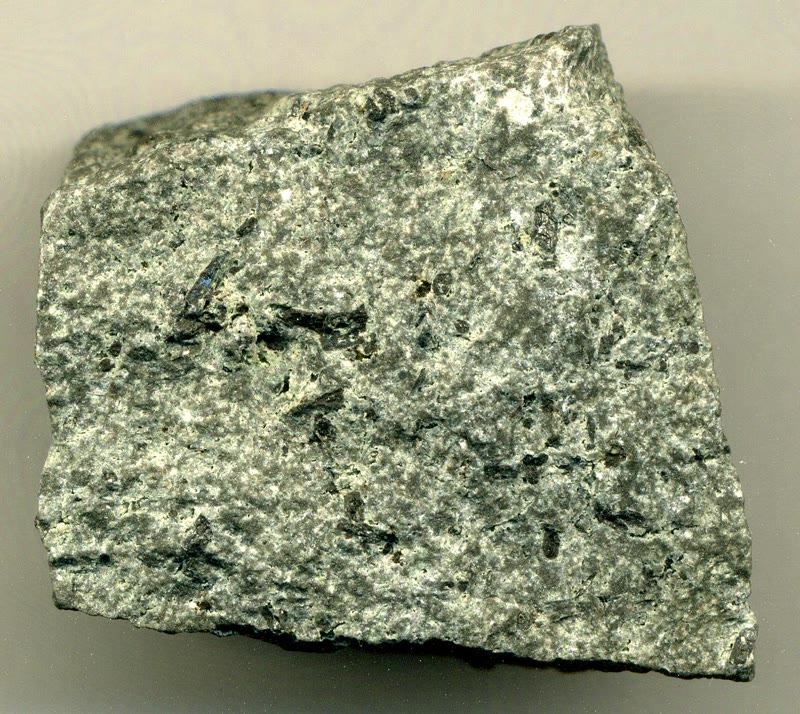
\includegraphics[height=4.4cm]{images/book2/g12-stjohn-andesite.jpg}\hspace{0.03\linewidth}%
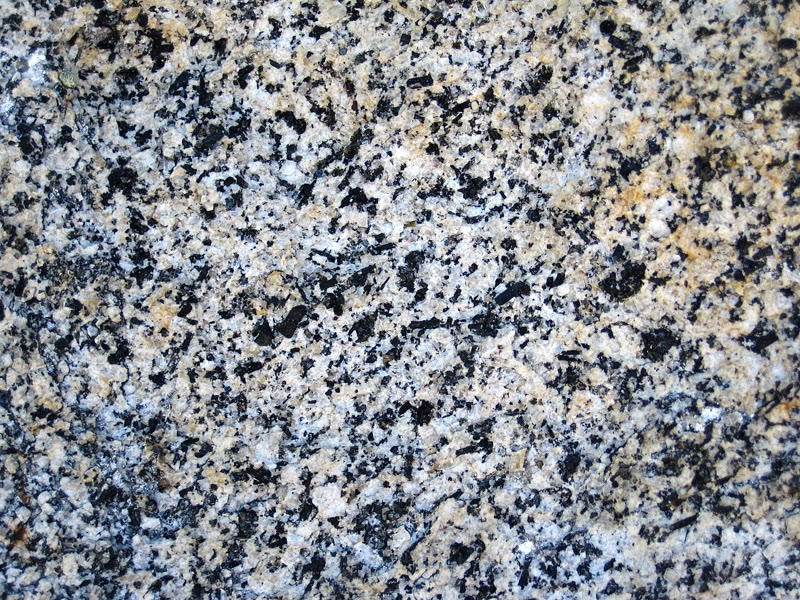
\includegraphics[height=4.4cm]{images/book2/g12-stjohn-granodiorite.jpg}

{\small Left: \omterm{def:g11:igneous-rocks:rock-names}{andesite}, a fine-grained \omterm{def:g11:igneous-rocks:volcanic-plutonic}{volcanic rock} of arcs. Right:
\omterm{def:g12:subduction-magmatism:granodiorite}{granodiorite} of the Sierra Nevada, with white plagioclase, grey quartz and
black biotite and hornblende. Photographs James St.~John (CC~BY~2.0).}
\end{omfigure}
% ledger: photo:g12-andesite, photo:g12-granodiorite

On average, the upper \omterm{def:g12:continental-crust:continental-crust}{continental crust} holds about \qty{67}{\percent}
\ce{SiO2}: it is \omterm{def:g11:igneous-rocks:felsic-mafic}{felsic}, like the granites that arcs make in quantity in
their \omterm{def:g12:subduction-magmatism:batholith}{batholiths}.
% ledger: rg14:crust (upper crust SiO2 66.6 wt %), tulane:magma-types, tulane:intrusions

\begin{definition}[Batholith]\label{def:g12:subduction-magmatism:batholith}
A \emph{batholith}\index{batholith} is a large mass of \omterm{def:g11:igneous-rocks:volcanic-plutonic}{plutonic rock} that covers
more than \qty{100}{km^2} where erosion has exposed it. It forms where many
\omterm{def:g11:igneous-rocks:intrusion}{plutons}, intruded one after another, join beneath the surface.
\end{definition}
% ledger: earle:batholith, tulane:intrusions

One of the largest in the world, the Coast \omterm{def:g11:igneous-rocks:volcanic-plutonic}{Plutonic} Complex, runs along
the Pacific coast from the Vancouver region of western Canada to
south-eastern Alaska. The Sierra Nevada \omterm{def:g12:subduction-magmatism:batholith}{batholith} of California formed above a
\omterm{def:g11:subduction-zones:subduction}{subduction zone}; most of its granites in Yosemite crystallised in the
Cretaceous, 105 to 85 million years ago. The rocks above them were worn
away over millions of years, and the \omterm{def:g11:igneous-rocks:intrusion}{plutons} that cooled deep down now form
the mountains.
% ledger: earle:batholith, nps:yosemite, photo:g12-sierra-nevada (St. John description), ics:base.Cretaceous

\begin{omfigure}
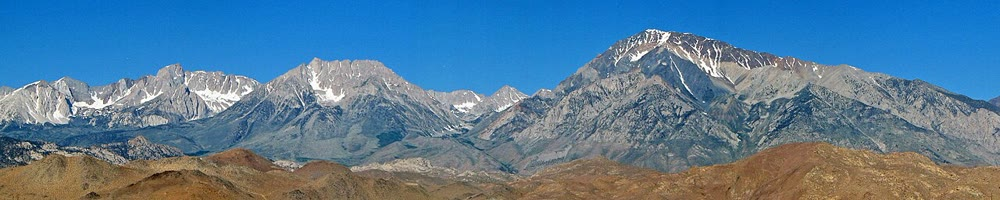
\includegraphics[width=0.94\linewidth]{images/book2/g12-stjohn-sierra-nevada-batholith.jpg}

{\small The Sierra Nevada, seen from the east: granite and \omterm{def:g12:subduction-magmatism:granodiorite}{granodiorite} of
the Sierra Nevada \omterm{def:g12:subduction-magmatism:batholith}{batholith}, which crystallised deep down above a
\omterm{def:g11:subduction-zones:subduction}{subduction zone} in the Cretaceous. Photograph James St.~John
(CC~BY~2.0).}
\end{omfigure}
% ledger: photo:g12-sierra-nevada, nps:yosemite

\section{How continents grow}

\begin{definition}[Continental growth]\label{def:g12:subduction-magmatism:continental-growth}
\emph{Continental growth}\index{continental growth} is the addition of new
\omterm{def:g12:continental-crust:continental-crust}{continental crust}, made from the mantle, mostly by the magmatism of arcs.
The net growth of the continents is that addition minus the \omterm{def:g12:continental-crust:continental-crust}{continental crust}
that returns to the mantle.
\end{definition}
% ledger: sv09:growth, ss09:balance

Arcs are where the light rock of the continents is made. Estimates of the
magma that arcs add today are about \qty{1.5}{km^3} a year at island arcs
and \qty{1.0}{km^3} a year at continental arcs; averaged over the long term,
about \qty{2.7}{km^3} a year. But \omterm{def:g11:subduction-zones:subduction}{subduction zones} also take \omterm{def:g12:continental-crust:continental-crust}{continental
crust} back into the mantle: sediment carried down with the \omterm{def:g11:subduction-zones:slab}{slab} and pieces
of the overriding plate scraped from beneath, about \qty{3.2}{km^3} a year.
The two are close, and the net growth of the continents over the last
several hundred million years may have been nil, or even negative.
% ledger: sv09:growth, ss09:balance

Continents also grow at their edges in another way. \omterm{def:g12:continental-crust:continental-crust}{Continental crust} is too
light to be subducted, so when a plate carries a continent into a trench the
two continents are welded together in a collision
(\cref{ch:g12:mountain-building}). Each continent has an old core, a \omterm{def:g12:continental-crust:craton}{craton},
surrounded by belts of younger rock, the deformed \omterm{def:g12:continental-crust:root}{roots} of former mountain
belts, added one after another at its edges
(\cref{ch:g12:continental-crust}).
% ledger: tulane:no-subduct (continental crust too buoyant to subduct), earle:collision, tulane:cratons

\section{Exercises}

\begin{exercise}[$\star$]\label{exo:g12:subduction-magmatism:1}
Give the word: (a) a line of volcanoes parallel to a trench, on the plate
that does not sink; (b) melting caused by adding water to a rock; (c) a
\omterm{def:g11:igneous-rocks:volcanic-plutonic}{plutonic rock} with more plagioclase than potassium feldspar and more than
\qty{20}{\percent} quartz; (d) a mass of \omterm{def:g11:igneous-rocks:volcanic-plutonic}{plutonic rock} larger than
\qty{100}{km^2}; (e) the addition of new \omterm{def:g12:continental-crust:continental-crust}{continental crust} made from the
mantle.
\end{exercise}

\begin{exercise}[$\star$]\label{exo:g12:subduction-magmatism:2}
On 18 May 1980 the ash column of Mount St.~Helens rose more than \qty{24}{km}
in less than 15 minutes. (1) What was its least mean rising speed, in
\unit{km/h} and in \unit{m/s}? (2) Compare it with the speed of the lateral
blast, at least \qty{480}{km/h}.
\end{exercise}

\begin{exercise}[$\star$]\label{exo:g12:subduction-magmatism:3}
Of the 1214 volcanoes of the catalogue active since the end of the last ice
age, 838 stand above a \omterm{def:g11:subduction-zones:subduction}{subduction zone}. (1) What percentage is that? (2) On
which side of a trench are these volcanoes? (3) Why are there none between
the trench and the volcanic front?
\end{exercise}

\begin{exercise}[$\star$]\label{exo:g12:subduction-magmatism:4}
A coarse-grained rock holds \qty{25}{\percent} quartz, \qty{45}{\percent}
plagioclase, \qty{15}{\percent} potassium feldspar and \qty{15}{\percent}
biotite and hornblende. (1) What fraction of its feldspar is plagioclase?
(2) Is it a \omterm{def:g12:subduction-magmatism:granodiorite}{granodiorite}?
\end{exercise}

\begin{exercise}[$\star$]\label{exo:g12:subduction-magmatism:5}
Give two reasons why the volcanoes of arcs erupt more explosively than those
of ridges.
\end{exercise}

\begin{exercise}[$\star\star$]\label{exo:g12:subduction-magmatism:6}
(1) A volcanic front lies \qty{150}{km} from its trench, above a \omterm{def:g11:subduction-zones:slab}{slab} that
dips at \ang{35}. How deep is the \omterm{def:g11:subduction-zones:slab}{slab} beneath it? (2) Compare with the
average of \qty{105}{km}.
\end{exercise}

\begin{exercise}[$\star\star$]\label{exo:g12:subduction-magmatism:7}
Take the \omterm{def:g11:subduction-zones:slab}{slab} to lie \qty{105}{km} beneath every volcanic front. How far from
the trench is the front when the \omterm{def:g11:subduction-zones:slab}{slab} dips at \ang{20}, and when it dips at
\ang{45}? What does that tell you about where to look for the arc?
\end{exercise}

\begin{exercise}[$\star\star$]\label{exo:g12:subduction-magmatism:8}
At \qty{100}{km}, the pressure is about \qty{3.16}{GPa}. (1) Using $T =
-5.104P^2 + 132.9P + 1120.7$ ($P$ in \unit{GPa}, $T$ in \unit{\celsius}),
compute the temperature at which dry \omterm{def:g11:ocean-ridges:peridotite}{peridotite} begins to melt there.
(2) With water, it begins to melt at about \qty{1000}{\celsius}. By how much
does water lower it? (3) The mantle wedge there is at, say,
\qty{1300}{\celsius}. Does it melt dry? Wet?
\end{exercise}

\begin{exercise}[$\star\star$]\label{exo:g12:subduction-magmatism:9}
The debris avalanche of Mount St.~Helens moved about \qty{2.5}{km^3} of
rock. Arcs add about \qty{2.7}{km^3} of new crust a year. (1) How many days
of the world's arc magmatism does the avalanche represent? (2) Why is the
comparison only a matter of size?
\end{exercise}

\begin{exercise}[$\star\star$]\label{exo:g12:subduction-magmatism:10}
(1) How much new crust do arcs add in a million years at \qty{2.7}{km^3} a
year? (2) The \omterm{def:g12:continental-crust:continental-crust}{continental crust} holds about \qty{9e9}{km^3}. How long would
arcs alone take to make that volume, if none of it were lost? (3) Compare with
the age of the Earth, 4.5 billion years.
\end{exercise}

\begin{exercise}[$\star\star$]\label{exo:g12:subduction-magmatism:11}
(1) In the section across Japan, why are many earthquakes shallower than
\qty{70}{km} left out when the \omterm{def:g11:subduction-zones:slab}{slab} is fitted? (2) The deep earthquakes lie
\qty{116}{km} down at \ang{140.5}~E and \qty{80}{km} at \ang{141.5}~E, with
\qty{86.4}{km} per degree. Compute the dip of the \omterm{def:g11:subduction-zones:slab}{slab}.
\end{exercise}

\begin{exercise}[$\star\star\star$]\label{exo:g12:subduction-magmatism:12}
Show that, for a front at distance $d$ from the trench above a \omterm{def:g11:subduction-zones:slab}{slab} of dip
$\theta$, the distance measured down the \omterm{def:g11:subduction-zones:slab}{slab} from the trench to the point
beneath the front is $d/\cos\theta$. For Japan ($d = \qty{270}{km}$,
$\theta = \ang{20}$), how long is it? The Pacific Plate moves towards
Japan at about \qty{83}{mm} a year; taking that speed all along the \omterm{def:g11:subduction-zones:slab}{slab}, how
long does a piece of sea floor take to travel from the trench to beneath the
volcanoes?
\end{exercise}
% ledger: usgs:tohoku (83 mm/yr)

\begin{exercise}[$\star\star\star$]\label{exo:g12:subduction-magmatism:13}
The magma chamber of Mount St.~Helens is about \qty{1}{km} wide and extends
from about 6 to \qty{14}{km} down. (1) Treating it as a vertical cylinder,
estimate its volume. (2) Compare it with the \qty{2.5}{km^3} of the avalanche.
(3) Compute the \omterm{def:g12:metamorphic-rocks:lithostatic}{lithostatic pressure} at its top and bottom ($\rho =
\qty{2830}{kg/m^3}$, $g = \qty{9.81}{m/s^2}$).
\end{exercise}

\begin{exercise}[$\star\star\star$]\label{exo:g12:subduction-magmatism:14}
Arcs add about \qty{2.7}{km^3} of crust a year, and \omterm{def:g11:subduction-zones:subduction}{subduction zones} take
back about \qty{3.2}{km^3}. (1) What is the net change per million years?
(2) Over 500 million years, what fraction of a crust of \qty{9e9}{km^3} is
that? (3) The authors call the net growth ``effectively nil''. Why, given
the uncertainty of each estimate?
\end{exercise}

\begin{exercise}[$\star\star\star$]\label{exo:g12:subduction-magmatism:15}
A \omterm{def:g12:subduction-magmatism:batholith}{batholith} exposes \qty{20000}{km^2} of \omterm{def:g12:subduction-magmatism:granodiorite}{granodiorite} whose \omterm{def:g11:igneous-rocks:intrusion}{plutons}
solidified between 5 and \qty{15}{km} down. (1) Estimate the volume of magma
it represents, taking it \qty{10}{km} thick. (2) At \qty{1}{km^3} a year,
the rate of all the world's continental arcs together, how long would they
take to make it? What does that tell you about the time over which a
\omterm{def:g12:subduction-magmatism:batholith}{batholith} is built?
(3) How much rock had to be eroded from above it before it could be seen?
\end{exercise}

\begin{problem}[{Weekend problem --- Beneath the volcanoes of Japan}]
\label{pb:g12:subduction-magmatism:1}
% ledger: data:b2-usgs-ne-japan, data:gvp, data:pb2002, sa06:slab-depth, hirschmann:solidus, wang20:wet-solidus, earle:arc-water, data:prem
% values (arc_magmatism.py): Megata 139.725, Iwate 141.001, trench 144.12; bins 140.5/141/141.5: 116.4/98.15/80.35 km; P_100km 3.157, dry_T_100km 1489
The volcanoes of north-east Japan between \ang{37.5} and \ang{40.5}~N lie
between \ang{139.7}~E (Megata, the westernmost) and \ang{141.0}~E (Iwate, the
easternmost); the Japan Trench lies at \ang{144.1}~E. The table gives the
median depth of the earthquakes deeper than \qty{70}{km} in three strips of
longitude, 1976--2025. Take \qty{111.2}{km} for one degree of latitude.

\begin{center}
\small
\begin{tabular}{|l|c|c|c|}
\hline
longitude (\unit{\degree}~E) & 140.5 & 141.0 & 141.5 \\ \hline
median depth (\unit{km}) & 116 & 98 & 80 \\ \hline
\end{tabular}
\end{center}

\medskip
\noindent\textbf{Part I --- The volcanic front.}
\begin{enumerate}
  \item Show that one degree of longitude at \ang{39}~N is about
        \qty{86.4}{km}.
  \item How far is the volcanic front from the trench?
  \item How wide is the arc, from Iwate to Megata?
  \item On which plate do the volcanoes stand, and on which side of the
        trench?
  \item Why are there no volcanoes between the trench and Iwate?
\end{enumerate}

\medskip
\noindent\textbf{Part II --- The earthquake section.}
\begin{enumerate}[resume]
  \item By how many kilometres do the median depths change from
        \ang{140.5} to \ang{141.5}~E?
  \item Over what horizontal distance?
  \item Compute the dip of the \omterm{def:g11:subduction-zones:slab}{slab}.
  \item Continue the line from \ang{141.0}~E, \qty{98}{km}, up to the
        surface. Where does it reach it, and how far is that from the trench?
  \item Suggest why the \omterm{def:g11:subduction-zones:slab}{slab} is less steep near the trench than deeper down.
\end{enumerate}

\medskip
\noindent\textbf{Part III --- The slab beneath the volcanoes.}
\begin{enumerate}[resume]
  \item Compute $H = d\tan\theta$ with the distance of question 2 and a dip
        of \ang{20}.
  \item Compare it with the median depth beneath the front.
  \item Compare both with the world range, 72 to \qty{173}{km}, and mean,
        \qty{105}{km}.
  \item How deep is the \omterm{def:g11:subduction-zones:slab}{slab} beneath Megata, using the line of question 9?
  \item Taking the crust of the arc to be about \qty{35}{km} thick, is the
        top of the \omterm{def:g11:subduction-zones:slab}{slab} beneath the front in the crust or in the mantle? How
        far below the base of the crust is it?
\end{enumerate}

\medskip
\noindent\textbf{Part IV --- Where the water comes from.}
\begin{enumerate}[resume]
  \item Where did the water of the \omterm{def:g11:subduction-zones:slab}{slab} enter its rocks, and in which
        mineral is much of it held?
  \item At \qty{100}{km} the pressure is about \qty{3.16}{GPa}. Compute the
        dry solidus there with $T = -5.104P^2 + 132.9P + 1120.7$.
  \item With water, the solidus is between 950 and \qty{1000}{\celsius}.
        By how much does water lower it?
  \item Why can the cold \omterm{def:g11:subduction-zones:slab}{slab} itself not be the source of the magma?
  \item Sum up: how deep is the \omterm{def:g11:subduction-zones:slab}{slab} beneath the volcanic front of north-east
        Japan?
\end{enumerate}
\end{problem}
